%%
%% This is file `sample-manuscript.tex',
%% generated with the docstrip utility.
%%
%% The original source files were:
%%
%% samples.dtx  (with options: `all,proceedings,bibtex,manuscript')
%% 
%% IMPORTANT NOTICE:
%% 
%% For the copyright see the source file.
%% 
%% Any modified versions of this file must be renamed
%% with new filenames distinct from sample-manuscript.tex.
%% 
%% For distribution of the original source see the terms
%% for copying and modification in the file samples.dtx.
%% 
%% This generated file may be distributed as long as the
%% original source files, as listed above, are part of the
%% same distribution. (The sources need not necessarily be
%% in the same archive or directory.)
%%
%%
%% Commands for TeXCount
%TC:macro \cite [option:text,text]
%TC:macro \citep [option:text,text]
%TC:macro \citet [option:text,text]
%TC:envir table 0 1
%TC:envir table* 0 1
%TC:envir tabular [ignore] word
%TC:envir displaymath 0 word
%TC:envir math 0 word
%TC:envir comment 0 0
%%
%% The first command in your LaTeX source must be the \documentclass
%% command.
%%
%% For submission and review of your manuscript please change the
%% command to \documentclass[manuscript, screen, review]{acmart}.
%%
%% When submitting camera ready or to TAPS, please change the command
%% to \documentclass[sigconf]{acmart} or whichever template is required
%% for your publication.
%%
%%
\documentclass[manuscript,screen,review,format=acmsmall]{acmart}
%%
%% \BibTeX command to typeset BibTeX logo in the docs
\AtBeginDocument{%
  \providecommand\BibTeX{{%
    Bib\TeX}}}

%% Rights management information.  This information is sent to you
%% when you complete the rights form.  These commands have SAMPLE
%% values in them; it is your responsibility as an author to replace
%% the commands and values with those provided to you when you
%% complete the rights form.
\setcopyright{acmlicensed}
\copyrightyear{2025}
\acmYear{2025}
\acmDOI{XXXXXXX.XXXXXXX}
%% These commands are for a PROCEEDINGS abstract or paper.
\acmConference[Conference acronym 'XX]{Make sure to enter the correct
  conference title from your rights confirmation email}{June 03--05,
  2018}{Woodstock, NY}
%%
%%  Uncomment \acmBooktitle if the title of the proceedings is different
%%  from ``Proceedings of ...''!
%%
%%\acmBooktitle{Woodstock '18: ACM Symposium on Neural Gaze Detection,
%%  June 03--05, 2018, Woodstock, NY}
\acmISBN{978-1-4503-XXXX-X/2018/06}


%%
%% Submission ID.
%% Use this when submitting an article to a sponsored event. You'll
%% receive a unique submission ID from the organizers
%% of the event, and this ID should be used as the parameter to this command.
%%\acmSubmissionID{123-A56-BU3}

%%
%% For managing citations, it is recommended to use bibliography
%% files in BibTeX format.
%%
%% You can then either use BibTeX with the ACM-Reference-Format style,
%% or BibLaTeX with the acmnumeric or acmauthoryear sytles, that include
%% support for advanced citation of software artefact from the
%% biblatex-software package, also separately available on CTAN.
%%
%% Look at the sample-*-biblatex.tex files for templates showcasing
%% the biblatex styles.
%%

%%
%% The majority of ACM publications use numbered citations and
%% references.  The command \citestyle{authoryear} switches to the
%% "author year" style.
%%
%% If you are preparing content for an event
%% sponsored by ACM SIGGRAPH, you must use the "author year" style of
%% citations and references.
%% Uncommenting
%% the next command will enable that style.
%%\citestyle{acmauthoryear}


%%
%% end of the preamble, start of the body of the document source.
\begin{document}

%%
%% The "title" command has an optional parameter,
%% allowing the author to define a "short title" to be used in page headers.
\title{The Quest for Unification: A Survey of Hardware-Agnostic Machine Learning Systems}

%%
%% The "author" command and its associated commands are used to define
%% the authors and their affiliations.
%% Of note is the shared affiliation of the first two authors, and the
%% "authornote" and "authornotemark" commands
%% used to denote shared contribution to the research.
\author{Paul Dutton}
\authornote{Both authors contributed equally to this research.}
\email{paul.dutton@my.utsa.edu}
\orcid{1234-5678-9012}
%\author{G.K.M. Tobin}
%\authornotemark[1]
%\email{webmaster@marysville-ohio.com}
\affiliation{%
  \institution{University of Texas at San Antonio}
  \city{San Antonio}
  \state{Texas}
  \country{USA}
}

%\author{Julius P. Kumquat}
%\affiliation{%
%  \institution{The Kumquat Consortium}
%  \city{New York}
%  \country{USA}}
%\email{jpkumquat@consortium.net}

%%
%% By default, the full list of authors will be used in the page
%% headers. Often, this list is too long, and will overlap
%% other information printed in the page headers. This command allows
%% the author to define a more concise list
%% of authors' names for this purpose.
\renewcommand{\shortauthors}{Dutton et al.}

%%
%% The abstract is a short summary of the work to be presented in the
%% article.
\begin{abstract}
The fragmentation across machine learning system stacks—from high-level programming languages to hardware accelerators—creates significant barriers to research productivity and deployment efficiency. This survey examines how unifying technologies like MLIR, ONNX, and emerging solutions such as Modular's MAX and Mojo aim to address these challenges by providing hardware-agnostic abstractions without sacrificing performance, potentially democratizing access to cutting-edge ML capabilities across diverse hardware platforms.
\end{abstract}

%%
%% The code below is generated by the tool at http://dl.acm.org/ccs.cfm.
%% Please copy and paste the code instead of the example below.
%%
\begin{CCSXML}
<ccs2012>
 <concept>
  <concept_id>00000000.0000000.0000000</concept_id>
  <concept_desc>Do Not Use This Code, Generate the Correct Terms for Your Paper</concept_desc>
  <concept_significance>500</concept_significance>
 </concept>
 <concept>
  <concept_id>00000000.00000000.00000000</concept_id>
  <concept_desc>Do Not Use This Code, Generate the Correct Terms for Your Paper</concept_desc>
  <concept_significance>300</concept_significance>
 </concept>
 <concept>
  <concept_id>00000000.00000000.00000000</concept_id>
  <concept_desc>Do Not Use This Code, Generate the Correct Terms for Your Paper</concept_desc>
  <concept_significance>100</concept_significance>
 </concept>
 <concept>
  <concept_id>00000000.00000000.00000000</concept_id>
  <concept_desc>Do Not Use This Code, Generate the Correct Terms for Your Paper</concept_desc>
  <concept_significance>100</concept_significance>
 </concept>
</ccs2012>
\end{CCSXML}

\ccsdesc[500]{Do Not Use This Code~Generate the Correct Terms for Your Paper}
\ccsdesc[300]{Do Not Use This Code~Generate the Correct Terms for Your Paper}
\ccsdesc{Do Not Use This Code~Generate the Correct Terms for Your Paper}
\ccsdesc[100]{Do Not Use This Code~Generate the Correct Terms for Your Paper}

%%
%% Keywords. The author(s) should pick words that accurately describe
%% the work being presented. Separate the keywords with commas.
\keywords{Artificial Intelligence, Heterogenous Compute, Compilers, Frameworks, Programming Languages, Edge Compute, Spiking Neural Networks, ASICs, GPUs, TPUs, FPGAs}

\received{20 February 2007}
\received[revised]{12 March 2009}
\received[accepted]{5 June 2009}

%%
%% This command processes the author and affiliation and title
%% information and builds the first part of the formatted document.
\maketitle

\section{Introduction}

The dramatic rise of deep learning has created an unprecedented demand for specialized computing hardware. Modern AI software developers have to work with an increasing number of hardware platforms, software frameworks, and programming paradigms to stay on the cutting edge. The fragmentation often means that developers become tied into a specific ecosystem with difficulties changing these things, even within the same vendor. Expertise becomes siloed, and promising research directions might not get the attention they deserve due to a lack of compatible hardware support.

While General Purpose GPUs (GPGPUs) initially democratized AI research and still serve many well, the development of a newer generation of Application Specific Integrated Circuits (ASICs) for deep learning such as Tensor Processing Units (TPUs), Neural Processing Units (NPUs) which are sometimes referred to collectively as xPUs, along with specialized systems like those from Groq, Cerebras, and Graphcore. Each hardware requires a new instruction set, compiler toolchain, libraries, and programmer training. These hardwares typicall operate alongside a Central Processing Unit (CPU) in a heterogenous computing system where tasks are strategically divided among the most capable hardware for that task.

This hardware diversity creates many hardware and software challenges. Python, which is rather slow but easy to learn, is a common developing programming language for a lot of deep learning. Familiar libraries such as TensorFlow, PyTorch are easily accessible in its ecosystem and call to more better performing C++, CUDA, or other faster code underneath. When developers need functionality beyond what is immediately and obviously available from Python, typically the only option is to turn to writing your own C++ / GPU functions and kernels in a language that operates closer to the metal. Few developers possess the expertise in writing Parallel Thread Execution (PTX), Nvidia's assembly language, although it is common to need to do so for the best results.

Rapid prototyping might be done in Python and then for production code a different team entirely will rewrite much of the project in that higher-performance or domain-specific language (DSL); this causes production bottlenecks, new learning curves, and fragmentation.

This situation exemplifies what Hooker terms "The Hardware Lottery" \cite{TheHardwareLottery}—research directions are disproportionately influenced by available hardware and its accessibility. Many ideas might be theoretically viable, but if they don't align well with Nvidia's CUDA based hardware architecture, the ideas appear dead in the water. As we witness the development of new hardware that differs greatly from modern GPUs in efforts to address some of their shortcomings, the research community becomes more and more fragmented. Fragmentation and competition are indeed joined at the hip, even are we are as a research community largely focusing on the context of transformer based Large Language Models (LLMs) and the kinds of algorithmic operations that make them possible. Alternative paradigms like neuromorphic computing and analog approaches face even steeper adoption barriers as they fundamentally diverge from conventional digital architectures.

As the hardware landscape diversifies, the field needs unifying technologies that can bridge these gaps. This survey examines approaches that aim to provide hardware-agnostic abstractions without sacrificing performance. We will:

1. Analyze current ecosystem fragmentation and its impact on research and deployment
2. Examine model exchange formats and intermediate representations that facilitate cross-platform compatibility
3. Evaluate compiler technologies that abstract hardware complexity from developers
4. Survey the evolving hardware acceleration landscape
5. Assess unifying approaches, with particular focus on ONNX's success in model exchange and Modular's integrated MAX/Mojo stack
6. Discuss implications for future research and development in a heterogeneous computing environment

Through this analysis, we hope to provide insight into how the field might overcome fragmentation barriers to democratize access to cutting-edge ML capabilities across diverse hardware platforms.

\section{The Fragmentation Problem}

Fragmentation in the AI ecosystem manifests along multiple dimensions: hardware architectures, software frameworks, programming models, and deployment environments. As specialized hardware emerges to accelerate operations needed by newer models, software stacks must be substantially rewritten, often from the compiler level up, in order to leverage these capabilities. This creates a significant lag between hardware launches and their practical usability. Beyond technical barriers, economic and organizational factors further encourage developers to remain within familiar architecture stacks, as migration costs can be prohibitively high in terms of expertise development, code rewriting, and performance optimization.

\subsection{The Current AI Ecosystem}

The AI software landscape is dominated by a handful of frameworks, each with their own programming models and hardware compatibility profiles. TensorFlow, PyTorch, and more recently JAX provide comprehensive environments for model development, training, and deployment. These frameworks offer high-level abstractions that shield developers from underlying hardware complexity while providing options to introduce handwritten optimizing components.

Despite their capabilities, no single framework universally supports the full spectrum of computing platforms, from mobile processors to specialized ASICs, many of which remain only internally available to the companies that have developed them. Framework compatibility is typically strongest for mainstream hardware (x86 CPUs and NVIDIA GPUs) with varying levels of support for other platforms. This creates a stratified ecosystem where the most accessible tools work primarily with the most dominant hardware:

\begin{itemize}
    \item \textbf{NVIDIA GPUs} are supported by CUDA (introduced 2006), which has evolved into a comprehensive ecosystem of libraries (cuDNN, cuBLAS), profiling tools, and optimization frameworks. These dominate the market \cite{NvidiaDominanceYahoo}
    \item \textbf{AMD GPUs} are accessible through ROCm and HIP (Heterogeneous Interface for Portability), with the latter specifically designed to provide CUDA compatibility in efforts to bring developers over
    \item \textbf{Intel's} ecosystem leverages OneAPI as a unified programming model coinciding with its entry into the discrete GPU market. This Application Programming Interface (API) has brought the support of The Linux Foundation as an open-source direction for the market
    \item \textbf{Edge devices} are targeted through specialized frameworks like TensorFlow Lite, requiring additional model optimization and often complete redeployment pipelines
\end{itemize}

Performance-sensitive applications frequently require developers to directly access hardware-specific APIs. The financial stakes are substantial—with large-scale models running on thousands of GPUs, even modest efficiency gains can yield significant cost savings. For instance, techniques like kernel fusion implemented in FlashAttention \cite{FlashAttention} have delivered substantial performance improvements for transformer architectures by optimizing memory access patterns and computation scheduling specifically for GPU execution models.

\subsection{Vendor Lock In}

NVIDIA has established dominant market position in AI acceleration, with their CUDA ecosystem becoming the de facto standard for high-performance deep learning. This dominance creates several forms of lock-in:

\textbf{Toolchain Dependencies:} NVIDIA's comprehensive ecosystem includes libraries, profilers, and development environments that developers come to rely on\cite{Modular3}. These tools often have specific version interdependencies that complicate migration \cite{Modular4}.

\textbf{Hardware-Specific Optimizations:} Organizations frequently invest in developing highly optimized, hardware-specific implementations of performance-critical operations. DeepSeek, for example, achieved superior performance through custom PTX (Parallel Thread Execution) code specifically targeting NVIDIA hardware \cite{deepseekai2024deepseekv3technicalreport}, bypassing CUDA entirely. This investment in hardware-specific knowledge creates significant switching costs.

\textbf{Architectural Fragmentation:} Optimizations frequently target specific generations of hardware within the same vendor's lineup—code optimized for NVIDIA's H100 GPUs may require significant reworking for A100s \cite{ShahJay2024FFaA}, despite sharing the same fundamental architecture. This issue compounds across vendor boundaries.

\textbf{Selective Implementation of Standards:} While cross-platform standards like OpenCL theoretically enable hardware-agnostic development, their practical utility is limited by incomplete implementations. NVIDIA's OpenCL support, for example, notably excludes access to tensor cores\cite{Modular5}, specialized units that provide substantial acceleration for matrix operations central to deep learning \cite{MarkidisStefano2018NTCP}. This strategic limitation ensures that peak performance remains accessible only through vendor-specific programming models. This creates a significant knowledge investment that becomes a sunk cost, reinforcing lock-in even when alternative platforms emerge. Once teams have invested in developing this specialized expertise, the switching costs to another platform become prohibitively high, even if the alternative platform offers theoretical performance advantages.

\textbf{Proprietary Access Models for New ASICs:} Emerging AI-specific hardware like Google's TPUs, Cerebras's Wafer-Scale Engine, Groq's Tensor Streaming Processors (TSPs), and Tenstorrent's Grayskull processors typically operate through proprietary interfaces, often accessible only through cloud services or with significant customer commitments. This creates additional fragmentation as each platform requires distinct programming models and optimization strategies.

[FIGURE HERE FOR SHOWING WHY THESE NEW ASICS ARE DESIRABLE].

This multi-faceted lock-in reinforces "The Hardware Lottery" effect; not only are researchers and developers constrained by available hardware, but they become increasingly committed to specific vendors and architectures through accumulated expertise and optimization investments. Each migration consideration must weigh not just immediate porting costs but also the performance penalties of operating on less-optimized platforms.

\section{Model Exchanges and Framework Unification Approaches}

To address fragmentation in the AI ecosystem, the field has developed two complementary approaches: standardized model exchange formats that enable cross-framework compatibility, and unified programming frameworks that attempt to provide hardware-agnostic abstractions. These efforts represent critical infrastructure for reducing the switching costs between different hardware and software stacks.

\subsection{ONNX as a Standard Exchange Format}

It isn’t to say that the field is completely void of tools that are more or less standard, available, accessible, and useful. The Open Neural Network Exchange (ONNX) format has emerged as a cornerstone of interoperability in the fragmented AI ecosystem. By providing a standardized representation of computational graphs, operators, and weights, ONNX enables models to move between disparate frameworks and deployment environments. 


ONNX achieves this through three key components: (1) a well-defined operator specification covering common neural network operations, (2) an extensible computation graph representation that captures model topology and dependencies, and (3) a standardized serialization and storage format. This allows models trained in one framework to be deployed in another without retraining or substantial redevelopment.

The practical impact of ONNX has been substantial, creating pathways between previously isolated ecosystems. Models developed in PyTorch can be deployed in TensorFlow environments and vice versa, significantly reducing framework lock-in. This interoperability is particularly valuable in deployment scenarios, where hardware and software constraints might differ from training environments.

While ONNX has proven effective for mainstream model architectures, challenges remain for more experimental or specialized designs. Work done \cite{ONNXFailures} has identified several common failure modes, primarily stemming from framework-specific operations, data type incompatibilities, and handling of complex control flow structures. Despite these limitations, ONNX has established itself as a vital "glue" for the industry, enabling practical cross-framework compatibility for the majority of production use cases.

\subsection{Hardware Agnostic Framework Approaches}

Beyond model exchange, the field has seen numerous attempts to create programming frameworks that abstract away hardware specificity while maintaining performance. These frameworks take diverse approaches to the fundamental tension between hardware-specific optimization and cross-platform compatibility.

\subsubsection{Cross Platform APIs: OpenCL and SYCL}

Open Computing Language (OpenCL) launched as an early effort to unite parallel workload programming \cite{OpenCLLaunch} in heterogeneous systems. It does, however, offer targeting of GPUs, CPUs, FPGAs, and some work has even been done to integrate quantum processing into the project for heterogeneous computing \cite{QPU}. The standard offers a common abstraction model for many use cases.

Despite its ambitious goals and successes in uniting the field in many ways, OpenCL has faced significant practical limitations. Performance often lags behind vendor-specific programming models, and support for advanced hardware features can be incomplete. Notably, NVIDIA's OpenCL implementation lacks support for tensor cores \cite{Modular5}, creating a substantial performance gap compared to CUDA-based implementations for deep learning workloads. Furthermore, the collaborative "design by committee" approach has faced criticism for impeding innovation. Apple, an original proponent, eventually abandoned OpenCL in favor of its proprietary Metal framework to better support its custom silicon \cite{Modular5}.

Building on lessons from OpenCL, the Khronos Group developed SYCL, which takes an Embedded Domain Specific Language (eDSL) approach. Implemented as a C++ template library, SYCL maintains OpenCL's cross-vendor aspirations while providing a more modern programming model based on C++17 standards. SYCL has gained momentum as a foundation for other cross-platform initiatives, including Intel's OneAPI. OneAPI is offered from Intel as a competing open-source library set for high performance compute on many devices against OpenCL and CUDA. While Intel remains in charge, they offer support for many other devices, from CPUs to GPUs to FPGAs. \cite{OneAPICloud}














%%%%%%%%%%%%%%%%%%%%%%%%%%%%%%%%%
\subsubsection{Apache TVM}
 
Apache has its TVM, a machine learning compiler for CPUs, GPUs, and other accelerators that makes judicious use of auto-tuning in its optimizing steps to help target a wide range of hardware\cite{ChenTianqi2018TAAE}. Auto-tuning tests parameters for operations to find out what is actually best for that target platform. By removing some of this work from the programmer and automating ‘trial and error’ testing, the idea is that you should be able to get very good performance on a wide range of targets without manual fiddling.
It is also MLIR based, making interoperability between other tools using MLIR more possible through the use of shared dialects.


%%%%%%%%%%%%%%%%%%%%%%%%%%%%%%%%%














\section{Hardware Acceleration Landscape}

The AI hardware ecosystem has rapidly diversified beyond traditional CPUs and GPUs to include specialized accelerators. This diversification creates both opportunities for performance improvements and challenges for creating unified software systems. This section surveys the major hardware platforms driving AI workloads and examines how their architectural differences contribute to ecosystem fragmentation.

\subsection{General Purpose Hardware}

\subsubsection{Central Processing Units (CPUs)}

CPUs remain the foundation of computing systems, characterized by sophisticated control logic, high single-thread performance, and versatile I/O capabilities. Some begin to incorporate support for Single Instruction Multiple Data (SIMD) extensions like AVX-512 that can accelerate AI operations, although these are best offloaded to external dedicated devices.

While these can be used for AI directly, they often have few cores to work with which makes parallelization difficult. Instead, they are often the main orchestrating hardware for heterogeneous systems. This includes data management, scheduling, handling workloads with complex logic that don't work well on massively SIMD architectures such as GPUs, and providing a well-known and easily targeted platform for any other such needs.

\subsubsection{Graphics Processing Units (GPUs)}

Originally designed for rendering 3D graphics, GPUs have become the dominant platform for deep learning computation. A screen of many pixels offers a great landscape to develop and exploit parallelism, and GPUs excel in that area. Their architecture features thousands of relatively simple cores organized into compute units that execute the same instruction across multiple data elements, effectively implementing a massive SIMD paradigm. This architecture aligns naturally with the data-parallel nature of neural network operations, where identical computations are performed across large, $N$-dimensional tensors.

NVIDIA's CUDA platform, introduced in 2006, transformed GPUs from specialized graphics processors to general-purpose computing devices by providing accessible programming models and comprehensive library ecosystems. The resulting General-Purpose GPU (GPGPU) paradigm proved extraordinarily effective for deep learning workloads, which consist primarily of parallelizable matrix multiplications and similar operations.

GPUs also have adapted to this new role, with specialized hardware segments like Tensor Cores, incorporation of higher amounts of High Bandwidth Memory (HBM), interconnection technologies such as NVLink for multi-GPU systems, and support for increasingly common faster data types such as FP16 or INT8\cite{MicikeviciusPaulius2018MPT}.

\subsubsection{Tensor Processing Units (TPUs)}

Google's Tensor Processing Unit represents one of the earliest purpose-built AI accelerators. First deployed internally in 2015 and later made available through Google Cloud, TPUs feature a systolic array architecture specifically optimized for matrix multiplication operations central to deep learning. This architectural specialization enables higher computational density and energy efficiency compared to general-purpose processors at the cost of their ability to generalize.

TPUs popularized the utilization of the Bfloat16 data format which keeps a wide dynamic range whilst reducing precision. As these chips are intended to work in multi-TPU systems, special attention was given to collective communication operations and memory bandwidth to make large scale systems feasible.

While TPUs offer significant performance advantages for supported workloads, they remain accessible only through Google's cloud infrastructure, with programming models generally coupled to Google's TensorFlow ecosystem.

\subsubsection{Neural Processing Units (NPUs)}

Neural Processing Units have emerged as common accelerators for edge and mobile AI applications. AMD's XDNA architecture, Apple's Neural Engine, and various mobile SoC designs from Qualcomm and MediaTek all incorporate NPUs. These accelerators are typically integrated into System-on-Chip (SoC) designs alongside CPU cores, sharing I/O and memory subsystems. 

NPU architectures generally prioritize energy efficiency over raw performance, making them suitable for battery-powered devices. They often feature fixed-function units for common operations (convolution, activation functions) and optimized datapaths for reduced-precision computation. However, their programming models remain highly fragmented, with each vendor providing proprietary software stacks and limited interoperability.

\subsubsection{Enterprise Level Accelerators}

The market for data center AI acceleration has expanded dramatically beyond GPUs, with several companies developing specialized hardware for training and serving large models:

\textbf{Cerebras Wafer-Scale Engine} Cerebras takes an extreme approach to scaling, building processors that span an entire silicon wafer \cite{LieSean2023CADD}. This architecture eliminates traditional chip boundaries, providing massive on-chip memory and computational resources within a single device. While offering unprecedented scale, the architecture requires specialized programming models and cooling infrastructure.

\textbf{Groq Tensor Streaming Processor} Groq's architecture prioritizes deterministic execution through a novel approach to scheduling \cite{Groq}. Rather than dynamically assigning work to compute units, Groq's compiler generates a precise execution schedule known at compile time. This approach enables predictable performance and latency guarantees particularly valuable for inference workloads.

\textbf{Graphcore Intelligence Processing Unit (IPU)} The IPU architecture emphasizes fine-grained parallelism and in-processor memory to minimize data movement. Unlike GPUs, which execute identical operations across many data elements, IPUs support more flexible execution patterns suited to complex computational graphs with irregular structure.

\textbf{Intel Gaudi and GNA} Intel offers diverse AI acceleration options including Gaudi processors acquired from Habana Labs and the Gaussian and Neural Accelerator (GNA) for low-power speech and audio processing. This portfolio approach provides specialized solutions for different AI deployment scenarios but further contributes to ecosystem complexity.

[FIGURE HERE] shows the performance offered by many of these systems; highlighting the good idea of developing new ASICs for AI workloads. Competition can be good for many actors in the market, but proliferation still has an extraordinary number of hurdles to overcome if we are to see full integration of these new designs into the mainstream workflow, easy access for research and business, and the successes of these projects to leave a lasting impact on direction for the industry as a whole.

\subsection{Emerging Hardware Approaches}

Beyond conventional digital accelerators, several alternative computing paradigms are being explored for neural network acceleration:

\subsubsection{Field-Programmable Gate Arrays (FPGAs)}

FPGAs offer reconfigurable hardware that can be optimized for specific neural network architectures. This flexibility enables substantial power efficiency improvements compared to fixed-architecture processors, with studies reporting up to 10x better energy efficiency than GPUs for certain workloads \cite{MohaidatTamador2024ASoN}. FPGAs are particularly valuable for edge deployment scenarios with stringent power constraints or rapidly evolving model architectures. 

Despite these advantages, FPGAs face significant adoption barriers in AI workflows. Their programming complexity, lengthy synthesis times, and limited software ecosystem support restrict their mainstream use. Projects like ONNX-to-FPGA conversion tools \cite{ONNXFlow} aim to simplify deployment, but significant gaps remain compared to GPU software ecosystems.

\subsubsection{In and Near-Memory Computing}

The "memory wall"—the growing disparity between computation and memory access speeds—represents a fundamental bottleneck for neural network performance. In-memory computing architectures address this challenge by performing computations directly within memory arrays, dramatically reducing data movement costs \cite{LuWenbin2022BtB-}.

As models grow faster than our hardware capability and Moore's Law, engineers also look to novel ideas such as switched capacitors for matrix operations, analog computing \cite{MoolchandaniDiksha2021ACIo}, and computing in-memory or closer to it than we have previously \cite{10.1145/3571155} \cite{NiemierM.2024SDAt}.

\subsubsection{Neuromorphic Computing}

Neuromorphic architectures draw inspiration from biological neural systems, implementing computational models that more closely resemble brain function than conventional artificial neural networks. Spiking Neural Networks (SNNs) represent a prominent neuromorphic approach, using discrete, time-dependent spikes for information transmission rather than continuous activation values \cite{10.1145/3571155}. Sure, IBM has their NorthPole and Intel their Loichi line of chips that implement SNNs directly in silicon architecture, but these are inaccessible in innumerable ways (an architecture without a program counter is a difficult target for a compiler), and make the problems in the current landscape look like the mildest of roadblocks. The hardware to run these is vastly different from a GPU; while they are massively parallel, there is no traditional program counter as operation is effectively entirely asynchronous and event driven, and traditional program pipelines will not work.

These architectural differences make neuromorphic systems largely incompatible with mainstream AI software stacks. Most compilers and the tools that make them possible are designed for devices with common architectures (Von Neumann CPUs, Harvard for smaller DSP or microcontroller boards, GPUs being controlled by the CPU in a heterogenous environment). Compiler infrastructures including MLIR lack support for the asynchronous, event-driven computation models that neuromorphic hardware requires. This incompatibility exemplifies an extreme case of "The Hardware Lottery" \cite{TheHardwareLottery}, where potentially valuable approaches remain underexplored due to misalignment with dominant hardware paradigms.



%%%%%%%%%%%%%%








As we scale further into High Performance Computing for large models, the Single Instruction Multiple Data (SIMD) approach of our GPUs moves into Multiple Instructions Multiple Data (MIMD) environments and we see chips planning for this kind of asynchronous operation at the higher layers of abstraction, such as with TPUs, Groq's accelerators, SambaNova, and even HPC graph execution architectures such as the Intel Configurable Spatial Accelerator (CSA).






%%%%%%%%%%%%%%
\subsection{Implications for Unification}

The diversity of hardware architectures—from conventional CPUs and GPUs to specialized AI accelerators and emerging computing paradigms—presents profound challenges for creating unified software systems. Each platform offers unique performance characteristics and programming models, creating natural fragmentation in the ecosystem.

As we move from the Single Instruction Multiple Data (SIMD) paradigm of GPUs toward more asynchronous Multiple Instruction Multiple Data (MIMD) architectures like those in TPUs, Groq accelerators, and neuromorphic systems, the complexity of unification increases substantially. Even advanced compiler infrastructures like MLIR face fundamental limitations in spanning these architectural divides.

Still, this doesn’t mean that we can’t begin to plan for diverse hardware and future-proof our AI stacks. Cooperation between hardware designers and software algorithmic specialists can certainly help to make the path forward more clear \cite{ZhangHongbin2023CTiD}. Hardware-software co-design approaches that consider compilation pathways alongside architectural innovations may help bridge these gaps. However, as Hooker notes in "The Hardware Lottery" \cite{TheHardwareLottery}, architectural paradigms that lack accessible developer tools and programming models will likely remain underutilized regardless of their theoretical advantages.

\section{The Role of Compilers}

Compilers play a pivotal role in addressing hardware fragmentation by providing layers of abstraction between high-level programming models and diverse hardware targets. These tools take higher level code, parse it, often apply their own optimizations, and eventually target a hardware platform. Modern compiler infrastructures for AI workloads have evolved dramatically from traditional approaches, incorporating specialized intermediate representations, auto-tuning capabilities, and domain-specific optimizations. This section examines how compiler technologies contribute to unification efforts across the fragmented AI ecosystem.

\subsection{Compiler Intermediate Representations}

Intermediate Representations (IRs) form the cornerstone of modern compiler design, providing a standardized internal format that decouples front-end languages from back-end code generation. This separation enables a critical advantage: a single IR can support multiple source languages and target multiple hardware platforms, creating a many-to-many mapping that reduces implementation complexity. For instance, if we have some $m$ programming languages, and some $n$ target hardware platforms, without IRs we would need $m * n$ solutions to write any code for any platform. An intermediate reduces this drastically to $m + n$ for scaling.

\subsubsection{LLVM: The Foundation of Modern Compiler Infrastructure}

A famous example stands in LLVM. This originally stood for “Low Level Virtual Machine” but has since expanded to much more, leaving the name orphaned. This compiler infrastructure established many common patterns now fundamental to hardware-agnostic compilation. Many modern languages compile to this well-defined IR, leaving LLVM to handle a lot of the heavy lifting. The popular programming languages C and C++ (through the Clang compiler), Rust, Zig, Swift, and even parts of CUDA all target LLVM.

LLVM's architecture offers several key benefits for cross-platform development:
\begin{itemize}
    \item A language-agnostic IR that preserves program semantics while abstracting language-specific details
    \item A modular design allowing independent development of front-ends and back-ends
    \item Sophisticated optimization passes that operate on the IR, benefiting all supported languages
    \item A flexible target description system for modeling diverse hardware architectures
\end{itemize}


From there, LLVM can target any number of target devices such as CPUs from the ubiquitous x86 platform, ARM, PowerPC, and so on. This makes language development easy whilst creating a common space for compiler and language developers to work in. As new features come to the IR, they can ripple through the ecosystem. 

Despite these advantages, LLVM was primarily designed for conventional CPU targets with limited support for heterogeneous computing environments. Its IR lacks native representations for many operations central to deep learning, such as high-dimensional tensor manipulations, specialized activation functions, and distributed computation patterns. These limitations prompted the development of AI-specific compilation infrastructures.

\subsubsection{MLIR: Multi-Level Abstraction for AI Workloads}

Chris Lattner, who helped guide the development of LLVM, the Clang compiler, and Swift programming language (amongs many other projects), began a new IR project while working at Google Brain called the Multi Level IR, or MLIR, to help address many existing issues with LLVM and to address modern computing needs, with AI workloads in mind and extensibility to theoretically any challenge, such as quantum computing \cite{LattnerChris2021Msci}. By offering multiple levels of abstraction, the hope is to make more features available at many levels for all kinds of developers, unify development pipelines, and offer a more flexible system that can be better adapted to a wider range of hardware, new and future. MLIR dialects “cleanly separate domain-spec\cite{Modular8}. 

MLIR's dialect architecture defines domain-specific abstractions, operations, and type systems that can be progressively lowered through different levels of representation to offer a group of reusable behavior. This approach offers several advantages for heterogeneous AI compilation:
\begin{itemize}
    \item Domain-specific dialects can represent high-level operations (tensor contractions, convolutions) with rich semantic information
    \item Progressive lowering through multiple abstraction levels preserves optimization opportunities
    \item Common infrastructure reduces implementation duplication across AI frameworks
    \item Extensibility for new hardware architectures and programming models
\end{itemize}

The impact of MLIR has been substantial, with adoption across major AI frameworks including TensorFlow, PyTorch, and ONNX. Even NVIDIA has incorporated MLIR into its CUDA compilation stack, suggesting its emergence as a unifying technology for the field. MLIR's flexible architecture provides theoretical support for diverse targets including emerging paradigms like quantum computing, though practical implementations for many specialized architectures remain in early stages. It has been open-sourced and is a part of the LLVM Foundation.

Similarly, the Accelerated Linear Algebra (XLA) open-source compiler wants to be the standard for machine learning workloads. It is built off of its own IR, High-Level Optimizer (HLO); this project was a part of TensorFlow, and now JAX \cite{DemeureNestor2023HGca}. It currently targets a number of hardware including CPUs, GPUs, and TPUs and increasingly incoporates MLIR. The project has been developed alongside a proprietary version by Google who set the project up to target their own new TPU hardware. Chris Lattner of course was a part of that team for some time and has spoken about its successes and failures \cite{Modular8} and how that story shapes his current works. 

Later, OpenXLA launched as an open source version that is framework agnostic and broader in its ability to support tensor-computing hardware from many companies and incorporates even more MLIR into its stack. XLA still struggles to optimize ideally for Neural Networks, although it still performs well in the general case \cite{XLAArticle}.



%%%%%%%%%%%%%%%%%
TVM and XLA
%%%%%%%%%%%%%%%%%%







\subsection{AI-Specific Compilation Strategies}


Beyond intermediate representations, modern AI compilers incorporate sophisticated automated optimization techniques that help bridge the gap between hardware-agnostic programming and hardware-specific performance tuning.

\subsubsection{Auto-Tuning for Performance Portability} % T-Pain section (go watch his NPR Tiny-Desk concert though he's actually the GOAT

For AI specific tasks, we see the development of auto-tuning strategies in compilers that are able to automatically generate code for different architectures by optimizing parameters to satisfy some objective function, be it memory accesses or other aspects of performance. Industry standard compilers in non-AI areas such as the GCC compiler or Clang compiler might offer some 150-200 possible flags to be passed along for such work. Auto-tuning reduces the burden on developers to manually tune for every target platform, as this space of optimizations is handled for us at compile time. 

However, auto-tuning approaches face fundamental challenges. As with any traditional compiler optimization techniques, there are no guarantees of speedups. The parameter space for optimization grows exponentially with operation complexity, requiring sophisticated search strategies to explore efficiently. Traditional approaches—including exhaustive search, genetic algorithms, and simulated annealing—face trade-offs between tuning time and discovered performance \cite{AshouriAmirH2018ASoC}. Recent research has applied machine learning to predict performance rather than measuring it directly, potentially reducing tuning overhead.

Apache TVM exemplifies this approach, incorporating a sophisticated auto-tuning system that can automatically discover optimal implementations for tensor operations across diverse hardware targets \cite{ChenTianqi2018TAAE}. TVM's auto-tuner explores a parameter space for each operation (tile sizes, loop unrolling factors, thread allocation strategies) and measures actual performance to identify optimal configurations.

\begin{figure}[h]
  \centering
  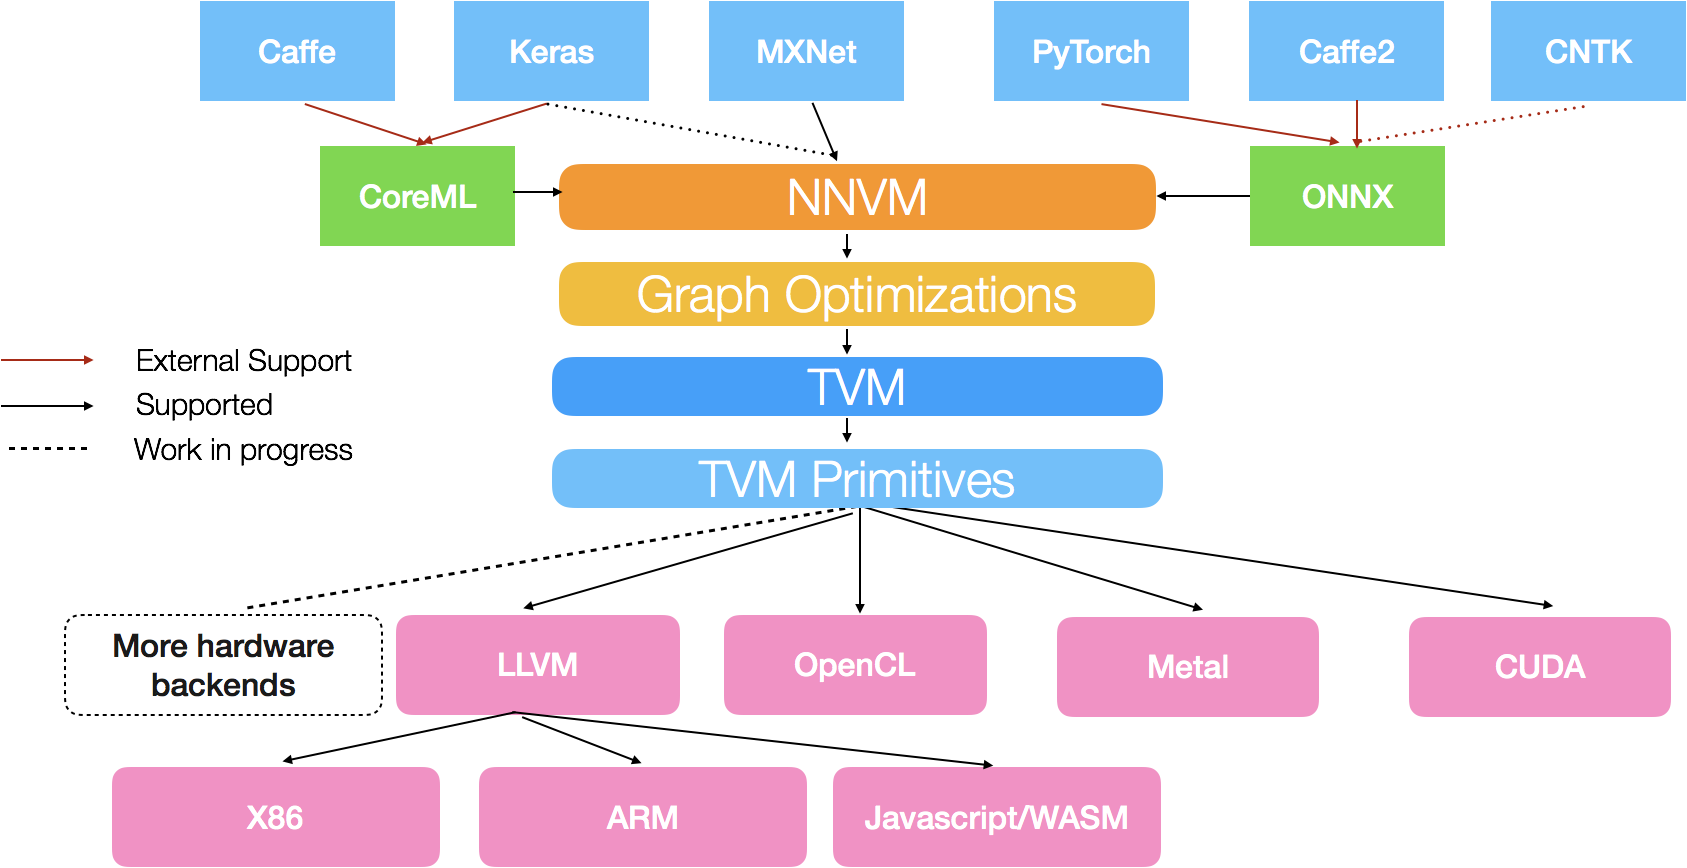
\includegraphics[width=\linewidth]{figures/nnvm_compiler_stack.png}
  \caption{What a modern ecosystem might look like.
    Apache TVM. (\url{https://tvm.apache.org/2017/10/06/nnvm-compiler-announcement}).}
  \Description{As an example, here we see where TVM comes into play, connecting many stages of the pipeline from high level libraries down to hardware.}
\end{figure}

\subsubsection{Heterogeneous Resource Allocation}

Advanced compilation strategies increasingly consider the entire heterogeneous system rather than individual accelerators in isolation. Projects like ZeRO-Offload demonstrate the potential of intelligent work distribution across CPUs and GPUs, moving appropriate computation and state management to CPUs to reduce GPU memory requirements \cite{RenJie2021ZDBM}.

This approach has been extended in systems like ZeRO-Infinity, which incorporates NVMe storage into the memory hierarchy for extremely large models \cite{RajbhandariSamyam2021ZbtG}. Such systems require sophisticated compiler analysis to determine optimal data placement and movement strategies based on hardware characteristics, including memory capacities, bandwidth limitations, and compute capabilities across the system.

\subsection{Domain Specific Languages}

Domain-Specific Languages (DSLs) represent another approach to addressing fragmentation by providing specialized programming models tailored to particular domains while abstracting hardware details. For AI workloads, several DSLs have emerged offering different trade-offs between expressiveness, performance, and hardware coverage.

\subsubsection{Standalone DSLs: Triton}

OpenAI has proffered Triton\cite{Triton}, a Python-like language that allows for efficient GPU programming without dipping into another language for kernels, addressing the "Two Language Problem". Based around its own LLVM "Triton-IR" that can compile to PTX and other targets, it claims performance near CUDA first-party libraries. They suggest that in many situations, performance can be faster than writing CUDA kernels in general practice due to its ease of use that helps offset the years of experience needed to write those top-performing CUDA kernels. Others suggest average performance degradations of about 20\% over the best hand-tuned kernels and first party libraries \cite{Modular7}.

Triton's compiler implements sophisticated optimizations including:
\begin{itemize}
    \item Automatic memory coalescing for efficient GPU memory access patterns
    \item Shared memory management without manual synchronization
    \item Automatic scheduling within GPU Streaming Multiprocessors (SMs)
\end{itemize}

\begin{figure}[h]
  \centering
  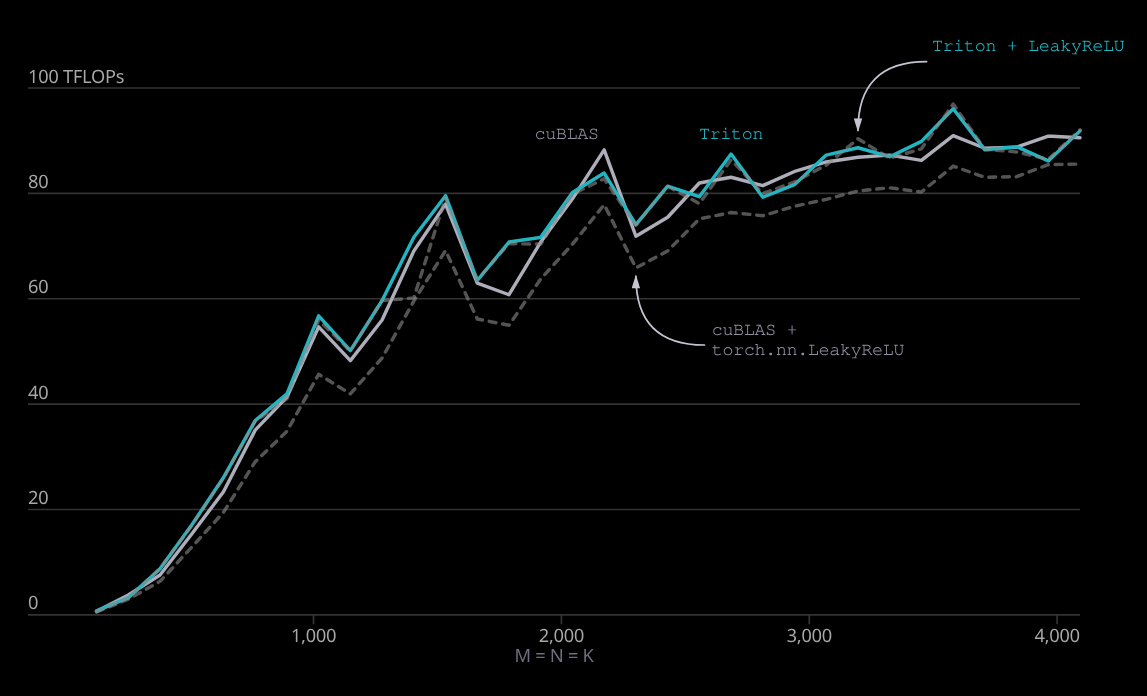
\includegraphics[width=\linewidth]{figures/tritonperformance.png}
  \caption{"V100 tensor-core performance of matrix multiplication with appropriately tuned values for $BLOCK_M$, $BLOCK_N$, 
  $BLOCK_K$, $GROUP_M$." (\url{https://openai.com/index/triton/}).}
  \Description{Things and stuff to replace here.}
\end{figure}

\subsubsection{Embedded DSLs for AI}


\textbf{JAX} stands for the combination of Just-In-Time-Compilation, Autograd (automatic differentiation of functions), and Accelerated Linear Algebra (XLA / OpenXLA). It is a Python library and eDSL that seeks to provide a set of composable function transformations for numerical computing. JAX, coming from Google, leverages XLA as its compilation backend, enabling deployment across CPUs, GPUs, and TPUs without code changes.

\textbf{SYCL} Developed by the Khronos Group, SYCL enables single-source heterogeneous programming in C++. Unlike OpenCL, which requires separate host and device code, SYCL integrates device computation within standard C++ syntax. Intel's Data Parallel C++ (DPC++) extends SYCL with additional features for Intel hardware.

\textbf{xDSL} Built on MLIR's extensible architecture, xDSL provides a framework for creating domain-specific dialects and transformations. This approach enables specialized languages to leverage MLIR's compilation infrastructure while maintaining domain-specific abstractions.

\textbf{Keras} Provides an interface for describing model graphs

Embedded DSLs offer several advantages for unification efforts:
\begin{itemize}
    \item Familiar syntax reduces the learning curve for domain specialists
    \item Integration with host language ecosystems provides access to existing tools and libraries
    \item Compilation to intermediate representations enables hardware-agnostic deployment
\end{itemize}

However, these approaches often face challenges in error reporting, debugging, and performance predictability compared to standalone languages, as the embedding can obscure the relationship between source code and generated implementation.

\subsection{Challenges and Limitations}

Despite significant progress, compiler-based approaches to fragmentation face fundamental challenges:

\begin{itemize}
    \item \textbf{Performance vs. Portability:} Hardware-specific optimizations often depend on architectural details that cannot be fully abstracted without performance penalties
    
    \item \textbf{Representation Gaps:} Existing IRs may lack efficient representations for emerging computation patterns such as sparse operations, asynchronous execution, or quantum algorithms
    
    \item \textbf{Hardware-Software Co-Evolution:} New hardware architectures often introduce capabilities that existing compiler infrastructures cannot effectively utilize
    
    \item \textbf{Standardization Complexity:} As with many standardization efforts, the proliferation of "unifying" compiler approaches can ironically increase fragmentation
\end{itemize}

Other projects exist, such as HTVM's \cite{JosseVanDelm2024HENN} compiler for Edge devices, ONNC \cite{ONNC} for connecting ONNX to accelerators, the HPVM framework and IR \cite{EjjehAdel2022HHPf} and many many more \cite{DeepLearningCompilerSurvey}. This list is non-exhaustive. Each attempt to create a universal standard paradoxically risks contributing to further fragmentation. a phenomenon sometimes called the "XKCD 927 Problem" \cite{xkcd}, where new standards increase fragmentation rather than consolidate.

These challenges highlight the need for coordinated ecosystem development that considers hardware capabilities, programming models, and compilation infrastructure as an integrated system rather than independent components.

\section{Unifying Approaches and Vertical Integration}

The preceding sections have examined multiple dimensions of fragmentation in the AI ecosystem and various approaches to address specific aspects of this challenge. Model exchange formats like ONNX address interoperability at deployment time, compiler infrastructures like MLIR provide abstraction layers for hardware targeting, and programming models like JAX offer unified interfaces for heterogeneous computation.

Despite these efforts, no single horizontal unification approach has fully resolved the fundamental tensions between hardware-specific optimization and cross-platform compatibility. 

This persistent challenge has led to growing interest in vertical integration approaches that address fragmentation by providing tightly-coupled solutions across the entire stack from programming language to hardware targeting. Rather than attempting to bridge diverse ecosystems horizontally, vertical integration creates cohesive pathways through the stack for specific use cases.

Modular's MAX and Mojo system represents one of the most ambitious recent attempts at vertical integration for AI workloads. By examining this approach in detail, we can better understand both the potential benefits and limitations of comprehensive stack integration as a response to ecosystem fragmentation.

\section{Modular's Approach: Vertical Integration} \label{sec:modular}

The preceding sections have examined various horizontal unification approaches—model exchange formats, compiler infrastructures, and hardware abstraction layers—each addressing specific aspects of ecosystem fragmentation. While these approaches offer valuable benefits, they operate within the constraints of existing ecosystem boundaries rather than fundamentally reshaping them.

Vertical integration represents an alternative unification strategy: rather than bridging diverse systems, it creates a cohesive technology stack spanning from programming language to hardware targeting. This section examines Modular's MAX and Mojo system as a case study of comprehensive vertical integration in AI infrastructure.

\subsection{Vertical Integration Approaches}

The persistent challenges of horizontal unification across the ecosystem have prompted interest in vertical integration approaches that connect the entire stack from programming language to hardware targeting. These approaches sacrifice ecosystem breadth for depth, providing tightly integrated solutions for specific scenarios.

Vertical integration offers potential advantages:
\begin{itemize}
    \item Consistent abstractions across the stack
    \item Optimization opportunities across layer boundaries
    \item Unified developer experience without API fragmentation
\end{itemize}

However, such approaches face significant adoption barriers, requiring developers to commit to a particular stack potentially at the expense of ecosystem compatibility.

\subsection{Modular}

Chris Lattner has taken his experience from working on various relevant areas (compilers, programming languages, hardware, MLIR, and so on) to found the company, Modular. They offer a totally integrated system starting with their own high-level programming language all the way through an enterprise platform for Kubernetes on the cloud or your own on-premise hardware.

As illustrated in Figure \ref{figure:maxgood}, the Modular system comprises three key components:
\begin{itemize}
    \item \textbf{Mojo} - A Python-compatible programming language with systems programming capabilities
    \item \textbf{MAX Engine} - A compiler and runtime system for AI workloads
    \item \textbf{MAX Serve} - Deployment infrastructure for model serving
\end{itemize}

This architecture incorporates model development, optimization, and deployment within a unified framework, eliminating many of the integration challenges that arise in pieced-together solutions. The system targets deployment across diverse environments including cloud infrastructure and on-premise hardware.

\begin{figure}[h]
  \centering
  \includegraphics[width=\linewidth]{figures/github-max.png}
  \caption{Complete picture of Modular systems.
    Modular MAX Github. (\url{https://github.com/modular/max}).}
  \Description{Here we can see the fully integrated pipeline for a user sending requests to a MAX Serve container; this includes more than the typical framework and has its MAX Engine and Mojo language working in the cloud (for this particular example) to run on a number of hardware.}
  \label{figure:maxgood}
\end{figure}

\subsection{Mojo Language}

The Mojo programming language represents a novel approach to the "two-language problem" faced by AI developers. Rather than accepting the division between a high-level language for model development and low-level languages for performance optimization, Mojo seeks to span this divide within a single language. Mojo is a language built almost as just a front-end to MLIR in order to take advantage of all that it offers. In that way, the Modular team sees the language as a necessary step in their quest to offer a complete and unified platform.

For most functionality, developers will not need to learn anything new. A valid Python program should be a valid Mojo program. The language is different from the common CPython reference implementation of Python in that instead of being interpreted, it’s compiled. This means no dipping into C++ for performance, no learning a new language, and a unified developer experience.

\subsubsection{Language Design and Python Compatibility}

To help entice programmers over even further, any and all existing Python code and libraries can be imported and used as-is without tinkering. The process is painless. You can continue to use PyTorch, JAX, or whatever you’ve developed without modification. At some point in the future, they hope to bring some of the Mojo improvements to Python to any imported library. This means switching to Mojo should be a no-brainer in most cases. This compatibility enables several key benefits:

\begin{itemize}
    \item Existing Python libraries can be imported and used directly
    \item Python developers can incrementally adopt Mojo features
    \item Organizations can leverage existing Python codebases without rewriting
\end{itemize}

\subsubsection{Systems Programming Capabilities}

Beyond Python compatibility, Mojo introduces several features more commonly associated with systems programming languages:

\begin{itemize}
    \item Static typing with type inference
    \item An ownership model for memory management inspired by Rust
    \item Compile-time metaprogramming through parameter specialization, inspired by Zig
    \item Native SIMD vectorization and parallelization primitives
\end{itemize}

These features enable performance-critical code to be expressed directly in Mojo rather than requiring implementation in separate C++ or CUDA modules, and they compose to offer powerful compiler optimizations. By exposing systems-level capabilities through a Python-compatible syntax, Mojo aims to make performance optimization accessible to a broader range of developers.

\subsubsection{Performance Characteristics}

Performance of the language is comparable to the kinds of ‘second’ languages called by Python traditionally for where performance matters. In comparison to stock Python, the performance gains can be massive. It offers tools for auto-tiling, auto-tuning, compile-time tuning, auto-vectorization, auto-parallelization, and so on. The tools will hopefully continue to mature.

Table \ref{table:matmuls} illustrates this through a matrix multiplication benchmark comparing various languages and compilers. This is a very naive example of matrix multiplication of square matrices; each bit of code was implemented and tested in very little time to get a feel for accessibility and expressivity. For some tests, we can say B is transposed in $A * B^T = C$, which makes for much more efficient memory access.

The benchmark demonstrates several key insights:
\begin{itemize}
    \item Unoptimized Python performs orders of magnitude slower than compiled alternatives
    \item Even optimized Python using NumPy (which calls into C++) remains substantially slower than native implementations
    \item Mojo achieves superior performance even compared to optimized C with OpenMP parallelization
\end{itemize}

Of course, the other languages can achieve better performance through use of Basic Linear Algebra Sublibraries (BLAS) libraries and the like, but this stands to show that Mojo gets you up and running with great performance and very little effort.

Code is available at \url{https://github.com/TheAgaveFairy/MatMulComparison}, the test platform is an AMD Ryzen 7 7600X CPU with DDR5 and Ubuntu 24.04.

%% do i need an appendix

\begin{table}[h]
    \caption{Comparison of Matrix Multiplications Across Languages / Compilers}
    \begin{tabular}{lll}
    Language / Compiler & Notes                    & Run Time us \\
    C / GCC             &                          & 3,075,132   \\
    C / GCC             & -O3, Transposed          & 142,836     \\
    C / GCC / OpenMP    & -O3, Transposed          & 28,612      \\
    C++ / Zig Clang     & 2D Vector                & 19,486,130  \\
    %C++ / Zig Clang     & -O3, 2D, Transposed      & 57,091      \\
    Go 1.23.6           &                          & 2,168,467   \\
    %Go 1.23.6           & Transposed               & 699,427     \\
    Python 3.12.8       & Native                   & 52,559,288  \\
    Python 3.12.8       & Numpy (C++), Transposed  & 1,196,449   \\
    Mojo 25.1.0         & -O3 (default), Transposed& 18,018      \\
    %Mojo 25.1.0         &                          &            
    \end{tabular}
    \label{table:matmuls}
\end{table}

\subsection{MAX Engine and Serve: Unified Compilation and Deployment}

While Mojo addresses programming model fragmentation, the Modular Accelerated Xecution (MAX) Engine and Serve components target compilation and deployment challenges in the AI ecosystem.

The MAX framework offers tools and libraries for model, kernel, and hardware developers. As a part of this, it offers a graph compiler, a runtime, and kernels. It also provides serving tools within containers for pipelining, scheduling, batching, and model loading. MAX wants to be a one-stop shop with the added benefit of having all of these under one roof.

\subsubsection{MAX Engine Architecture}

By building on MLIR, MAX Engine can leverage the dialect system to represent operations at multiple levels of abstraction. This enables both hardware-independent optimizations and hardware-specific code generation from a common representation. MAX Engine provides a unified compilation and runtime system for AI workloads across diverse hardware targets. Its architecture includes:

\begin{itemize}
    \item A graph compiler that optimizes high-level model representations
    \item Specialized kernel implementations for performance-critical operations
    \item A runtime system that manages execution across heterogeneous devices
\end{itemize}

A key architectural advantage is the direct integration between Mojo and MAX Engine. Rather than passing through multiple abstraction layers and conversion steps, Mojo code can be directly lowered to efficient implementation through MLIR, potentially preserving more semantic information for optimization.

\subsubsection{Hardware Targeting Strategy}

MAX Engine currently supports CPUs and NVIDIA GPUs, with AMD support under development. Notably, the system compiles directly to native code for each platform, generating PTX for NVIDIA GPUs without requiring the full NVIDIA toolkit or CUDA runtime. This approach offers several advantages:

\begin{itemize}
    \item Reduced deployment complexity and container size
    \item Elimination of version compatibility issues between CUDA components
    \item Potential for more comprehensive cross-compilation
\end{itemize}

This direct compilation strategy contrasts with approaches that rely on vendor-provided libraries and runtime systems, potentially reducing dependency on specific vendor ecosystems and their issues \cite{Modular4}.

\subsubsection{Deployment Infrastructure}

Early performance evaluations of the Modular stack show promising results compared to established solutions. Figures \ref{vllmthroughput} and \ref{vllmmetrics} compare MAX Engine against vLLM, a widely-used library for LLM serving, across several benchmark workloads.

These comparisons demonstrate that MAX Engine achieves competitive performance despite lacking specific optimizations like large batch support and paged attention\cite{maxgpu} that have been refined in vLLM. The performance metrics show particular strengths in GPU utilization and reduced non-kernel time, suggesting effective system-level optimization. These tools are still early in development.

It is worth mentioning the additional cluster system which aims to achieve large scale, multi-node systems \ref{figure:maxgood}. Of course, not only do we have to develop models, but we have to deploy them to customers as well. Offering this extra step could prove beneficial for developer ease.

\begin{figure}[h]
    \label{vllmthroughput}
  \centering
  \includegraphics[width=\linewidth]{figures/max-vs-vLLM.png}
  \caption{Comparison of MAX Engine vs. vLLM.
    Modular Blog. (\url{https://www.modular.com/blog/max-gpu-state-of-the-art-throughput-on-a-new-genai-platform}).}
  \Description{CAN I STEAL THIS CAPTION Request throughput of vLLM vs MAX with concurrent request limits of 248 and 512 requests on three benchmark workloads: ShareGPTv3, Sonnet Prefill-Heavy, and Sonnet Decode-Heavy. Each benchmark was run with 500 prompts.}
\end{figure}

\begin{figure}[h]
\label{vllmmetrics}
  \centering
  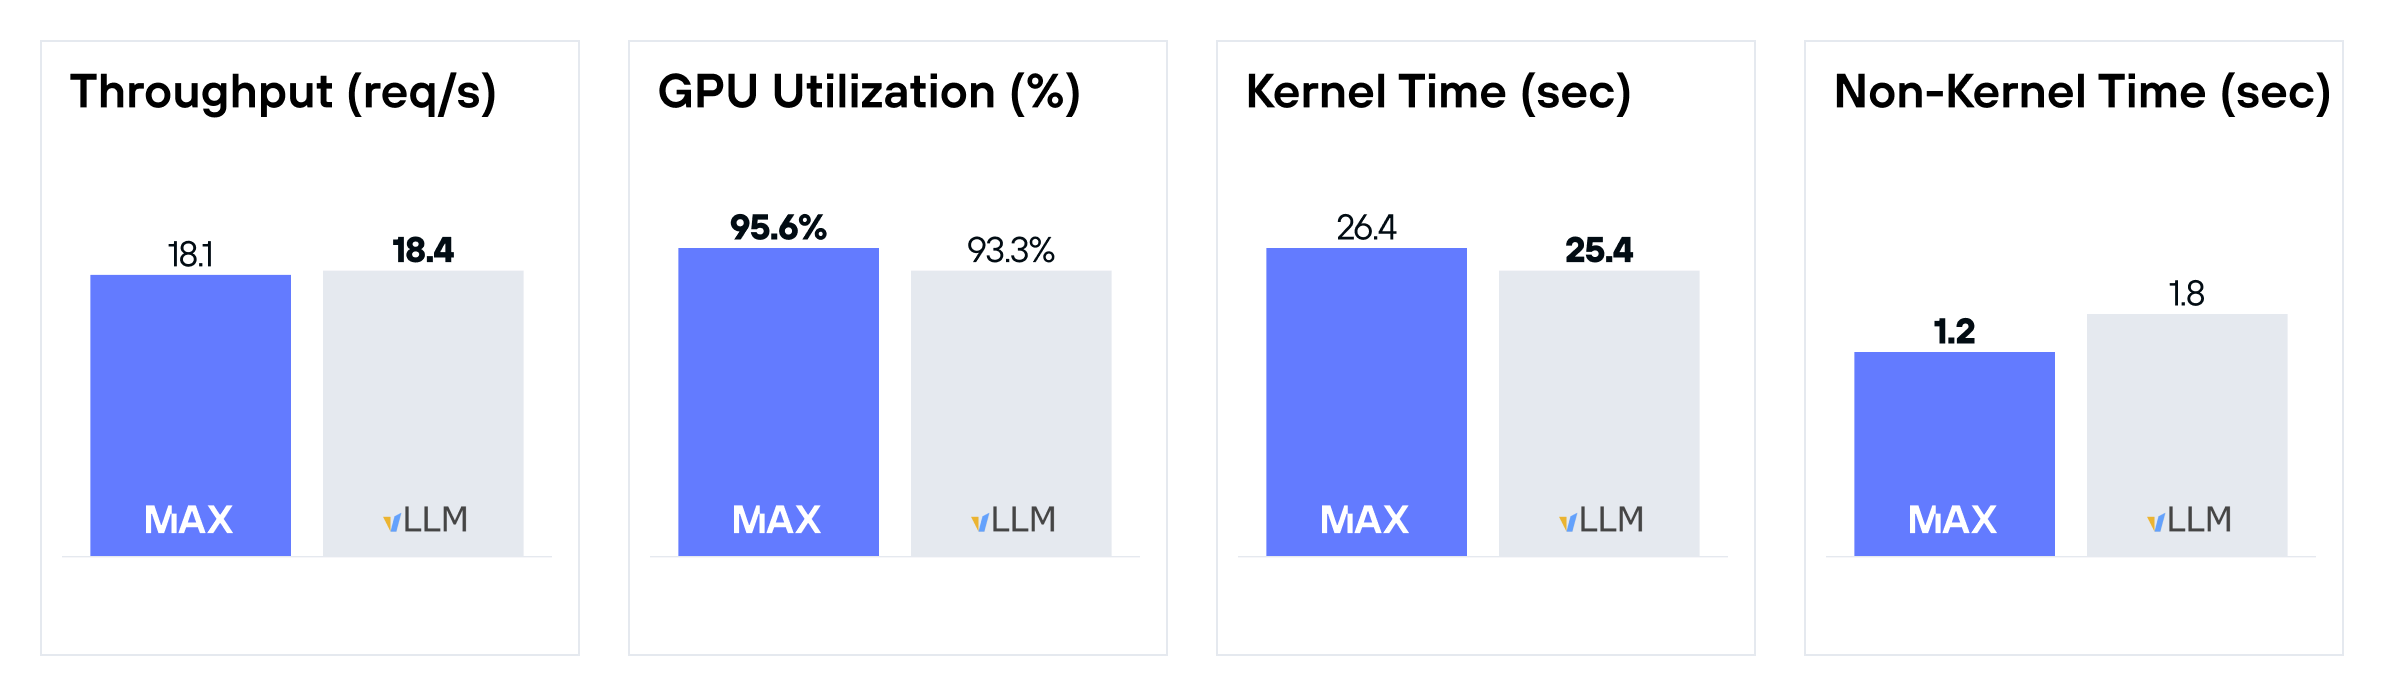
\includegraphics[width=\linewidth]{figures/max-vllm-gpu.png}
  \caption{Comparison of MAX Engine vs. vLLM.
    Modular Blog. (\url{https://www.modular.com/blog/max-gpu-state-of-the-art-throughput-on-a-new-genai-platform}).}
  \Description{CAN I STEAL THIS CAPTION Comparison of Performance Metrics on the ShareGPTv3 benchmarking workload for MAX vs vLLM. Detailed definitions of the performance metrics are in the citation. For request throughput and GPU utilization, higher is better. For Kernel Time and Non-Kernel Time, lower is better.}
\end{figure}


\subsection{Analysis: Trade-offs}

Modular's approach is no panacea, and does offer some drawbacks. Vertical integration can cause new kinds of fragmentation, lose flexibility, and fail in "eggs all in one basket" kinds of ways.

\subsubsection{Vertical Integration}

Modular's approach illustrates both the potential benefits and inherent limitations of vertical integration as a unification strategy. The integrated stack offers several advantages:
\begin{itemize}
    \item Elimination of abstraction gaps between components
    \item Unified optimization across traditional boundaries
    \item Consistent developer experience from programming to deployment
    \item Reduced dependency on multiple vendor ecosystems
\end{itemize}

However, this approach also involves significant trade-offs:
\begin{itemize}
    \item A new system still needs to be learned and adopted
    \item Potentially decreased flexibility to incorporate best-of-breed components from different vendors
    \item Increased commitment to a single technology stack
    \item Potential for feature lag compared to specialized solutions in rapidly evolving domains
\end{itemize}

The fundamental question for vertical integration approaches is whether the benefits of cohesion outweigh the costs of decreased interoperability with the broader ecosystem. For organizations struggling with the complexity of integrating fragmented components, a unified stack may offer substantial advantages despite these trade-offs. If nothing else, this undertaking should offer the industry great insights by providing a new radical paradigm.

The system's reliance on open standards like MLIR provides potential interoperability pathways with other ecosystem components, which may mitigate some of the limitations of vertical integration. This hybrid approach—unified internal architecture with standardized external interfaces—could represent a promising direction for addressing fragmentation while maintaining ecosystem connections.

\subsubsection{One Complicated Language}

Python offers many features and high level abstractions, making the feature set of Mojo already higher than simpler languages. Mojo adds functionality in order to tap into some key features of their MLIR based compiler, although this further increases complexity.

\begin{itemize}
    \item An ownership and lifetime system like Rust and Swift can be difficult to learn
    \item The addition of the $fn()$ keyword along with $def()$ for function declaration offers different behaviors to choose between
    \item Names (variables) may now only have one type, designated by that name's first assignment
    \item Separation of compile time \textbf{parameters} from runtime \textbf{arguments} allows for powerful metaprogramming, at the cost of additional syntax and complexity
    \item Extensive use of function declarations for functionality
    \item MAX Graph system is a new way to declare operations, marking a new transition for those used to languages like CUDA or Triton
\end{itemize}

While it may be that one only needs to learn a single language to reach all levels of performance, it is one language that has had to combine both the highest level abstractions of languages like Python as well as the low-level systems level control of C++ and Rust along with its own new ecosystem of MAX tools. Switching to this system will take work from both camps and the alleged benefit of having just one language becomes less obvious as the learning curve can be massive to leverage both ends of the spectrum provided.

\section{Conclusion}

There is a continuing challenge of hardware and software codesign. Much of the burden lands on compilers, and tools like MLIR certainly are going a long way in standardizing the dialects that everybody will "speak" as the tools are built to get our models running.

Layers of abstraction can make things very easy, but we still must consider the cost of performance for the sake of portability. The tradeoffs weigh differently for each party; research might need to move fast whilst an inference platform might want to fight for every last bit of performance they can to save dollars in their massive operations.

The development and emergence of new standards such as ONNX show important pieces of glue for the industry, and competition between frameworks offers a diverse approach to tackling big problems.

Unifying approaches such as a top-to-bottom rebuilding of our entire stacks from the ground up as seen in Modular are extraordinarily large tasks. If performance can't match other solutions, if compatibility can't be built deeply with other systems, if people don't want to learn yet another system, the project could be dead before it even starts. A one-size-fits all solution might be the best for nobody, as we need custom solutions to compete.

%\section{THINGS I STILL WANT TO TALK ABOUT}

%SYCL and OneAPI by Linux Foundation proposal;
%compilers kernel fusion;
% OpenVINO is another end-to-end solution for deploying inference of models across Intel hardware (and others, with more to come).
 
\bibliographystyle{ACM-Reference-Format}
\bibliography{mybibliography}

\end{document}
\endinput
%%
%% End of file `sample-manuscript.tex'.
